% lwocumentclass[10pt]{beamer} % 4/3 aspect ration works as well
\documentclass[10pt,aspectratio=169]{beamer}
%----------------------------------------------------------------------------------------
%	PACKAGES AND THEMES
%----------------------------------------------------------------------------------------

\makeatletter
\def\input@path{{EuXFEL_beamer_theme/}}
\makeatother

\mode<presentation>{
  \usetheme{EuXFEL}
  \usecolortheme{EuXFEL}
}
\usepackage{hyperref}
\usepackage{amsmath}
\usepackage{graphicx}
\graphicspath{{EuXFEL_beamer_theme/}{figures/}{./}}
\usepackage{helvet}
\usepackage[T1]{fontenc}
\usepackage{tikz}
\usetikzlibrary{shapes, arrows, calc, positioning}
\usetikzlibrary{decorations.pathreplacing}
\usepackage[spanish,provide=*]{babel}
\usepackage{amsmath,amssymb}%,amsthm,amsxtra,mathabx}
\usepackage{lipsum}
\usepackage{verbatim}
\usepackage{datetime}
\usepackage{multirow}
\usetikzlibrary{trees,arrows,positioning}

\definecolor{advancedcolor}{RGB}{255,140,0}    % Medium Orchid (purple)
\definecolor{basiccolor}{RGB}{0,70,140} % Dodger Blue

\tikzset{
    arrow/.style={->, >=stealth, thick}
}

% Text-only node styles with no shapes surrounding them
\tikzstyle{level1}=[font=\Large\bfseries, text centered]
\tikzstyle{level2}=[font=\large\bfseries, text centered, text=basiccolor!80!black]
\tikzstyle{level3}=[font=\normalsize\bfseries, text centered, text=advancedcolor!80!black]
\tikzstyle{endpoint}=[font=\small, text centered, text=black]

\renewcommand{\familydefault}{\sfdefault}
\renewcommand\mathfamilydefault{}
\newcommand{\colorbf}[1]{{\color{xOrange}\textbf{#1}}}

\newdateformat{dmydate}{%
    \twodigit{\THEDAY}~\monthname[\THEMONTH] \THEYEAR
%    \dayofweekname{\THEDAY}{\THEMONTH}{\THEYEAR} \twodigit{\THEDAY}~\monthname[\THEMONTH] \THEYEAR      
}   

\title[Aceleración de Hardware para un Robot Manipulador Móvil Omnidireccional Autónomo]{Aceleración de Hardware para un Robot Manipulador Móvil Omnidireccional Autónomo}

\author{Manuel Piña Olivas } % Your name
\institute[UACJ] % Your institution as it will appear on the bottom of every slide, may be shorthand to save space
{\noindent
  Asesor de Tésis\\% Your email address
  Dr. Franceso José García Luna\\
}
\date{\dmydate\today} % Date, can be changed to a custom date

\setbeamersize{text margin left=.05\pdfpagewidth,text margin right=.05\pdfpagewidth}

\begin{document}

{
  \setbeamertemplate{headline}{}
  \begin{frame}
    \titlepage
   \end{frame}
}

\begin{frame}{Artículos Principales de Investigación}
  \begin{enumerate}
      \item Model Based Approach for Automatic Generation of Hardware Architecture for Robotics.
      \item A General Inverse Kinematic Formulation and Control Schemes for Omnidirectional Robots.
      \item Virtual Teleoperation System for Mobile Manipulator Robots Focused on Object Transport and Manipulation.
      \item Autonomous Mobile Robot Path Planning Techniques - A Review: Classical and Heuristic Techniques.
  \end{enumerate}
\end{frame}

\begin{frame}{Model Based Approach for Automatic Generation of Hardware Architecture for Robotics \scriptsize{Ariel Podlubne, Johannes Mey, René Schöne, Uwe Aßmann, and Diana Göhringer}}
  Se presenta una manera de integrar múltiples aceleradores de hardware en un sistema robótico (independientemente del middleware usado).\\[5pt]
  
  \textbf{Problemáticas:}
  \begin{itemize}
    \item No existen interfaces entre software (ROS) y aceleración de hardware PL (FPGA).
    % \item No hay un enfoque sistemático para mapear mensajes de ROS a hardware.
  \end{itemize}

  \textbf{Propuestas:}
  \begin{itemize}
    \item Desarrollar una interface de comunicación entre software (ROS) y hardware (FPGA).
    \item Evitar cuello de botella de flujo de datos con el protocolo de comunicación AXIS.
  \end{itemize}

  \textbf{Resultado:}
  \begin{itemize}
    \item Plataforma móvil basada en FPGA con funcionalidades de ROS incorporadas.
  \end{itemize}
\end{frame}

\begin{frame}{Protocolos de Comunicación}
  \begin{columns}[onlytextwidth]
    \begin{column}{0.5\textwidth}
      \begin{center}
        \begin{figure}
          \begin{center}
            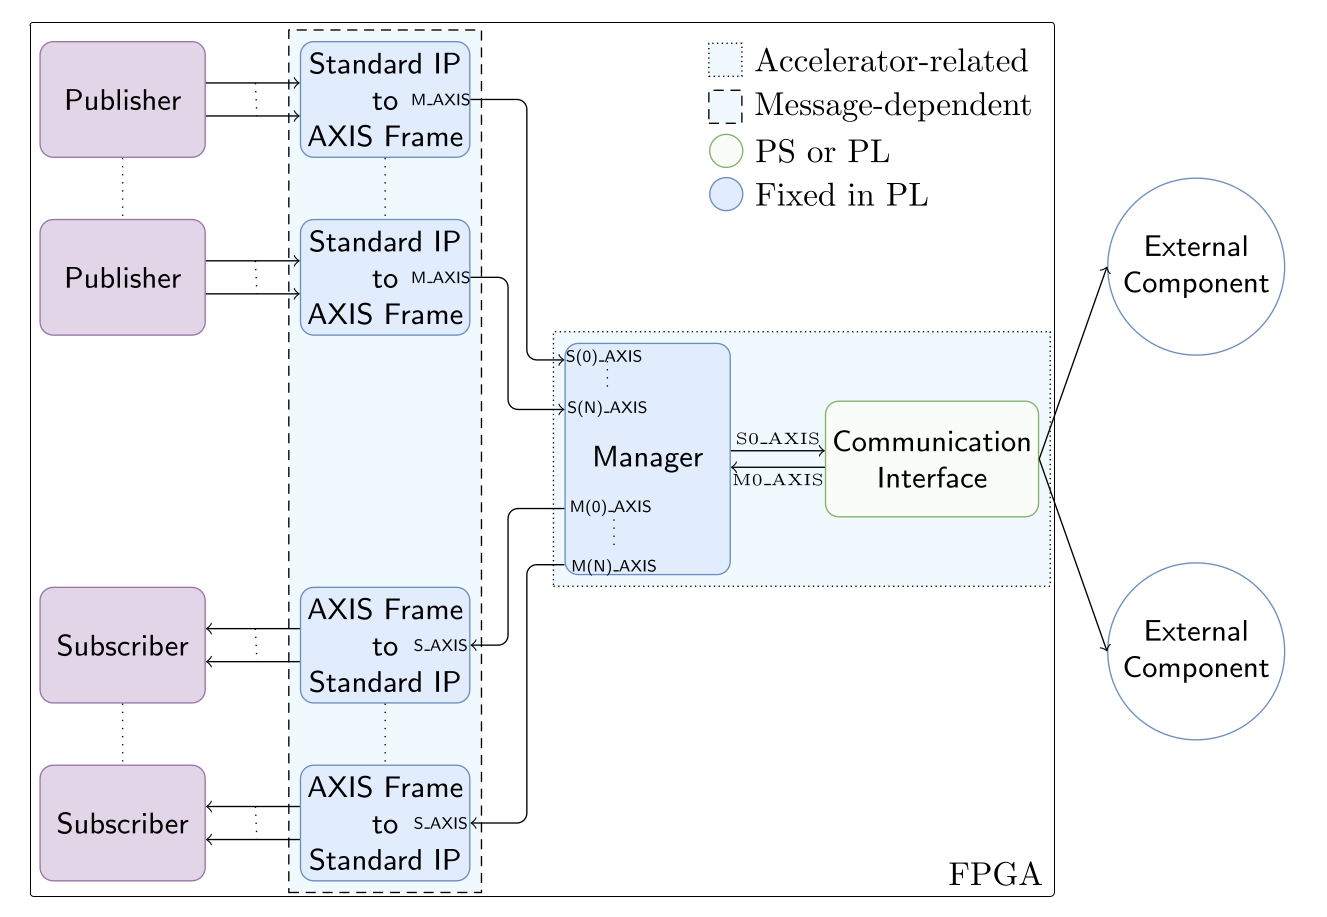
\includegraphics[width=0.95\textwidth]{figures/axis.png}
          \end{center}
          \caption{Protocolo AXIS}\label{fig:axis}
        \end{figure}
      \end{center}
    \end{column}
    \begin{column}{0.5\textwidth}
      \begin{figure}
        \begin{center}
          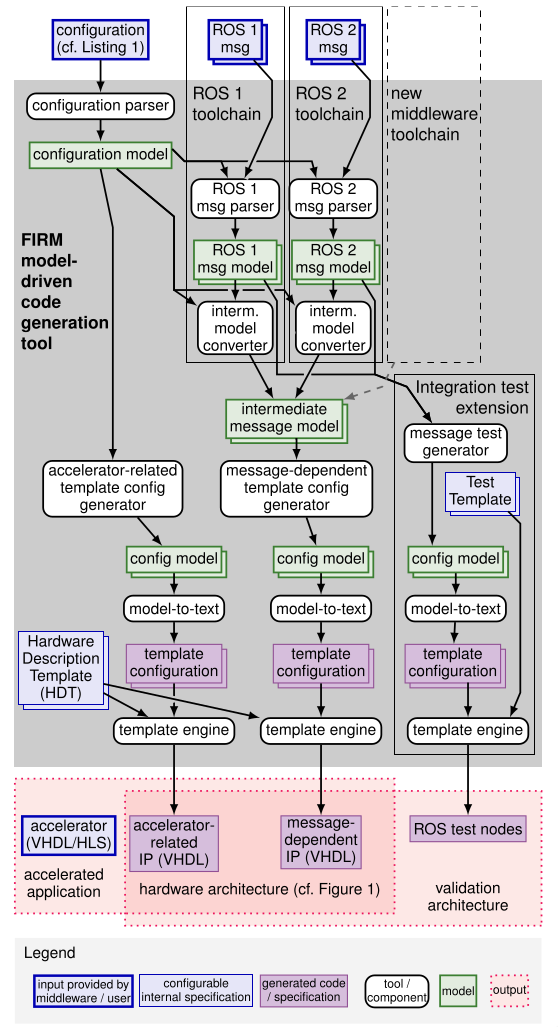
\includegraphics[width=0.42\textwidth]{figures/flow-chart.png}
        \end{center}
        \caption{Diagrama de Flujo}\label{fig:flowchart}
      \end{figure}
    \end{column}
  \end{columns}
\end{frame}

\begin{frame}{Autonomous Mobile Robot Path Planning Techniques-A Review: Classical and Heuristic Techniques \scriptsize{Mubarak Badamasi Aremu, Ibrahim K. Kabir, Gamil Ahmed and Sami El-Ferik}}
  Un robot móvil autónomo (AMR) es un tipo de robot que puede comprender y navegar sus alrededores por sí mismo.\\

  \textbf{Problemáticas:}
  \begin{itemize}
    \item Encontrar una ruta óptima sin colisiones hasta el destino deseado.
  \end{itemize}

  \textbf{Propuestas:}
  \begin{itemize}
    \item Categorizar algoritmos de planificación de rutas.
  \end{itemize}

  \textbf{Resultado:}
  \begin{itemize}
    \item Clasificación de métodos en distintas categorías. 
    \item Ejemplo de aplicaciones para distintas necesidades.
  \end{itemize}
\end{frame}

\begin{frame}{Taxonomía de Técnicas de Planificación}
  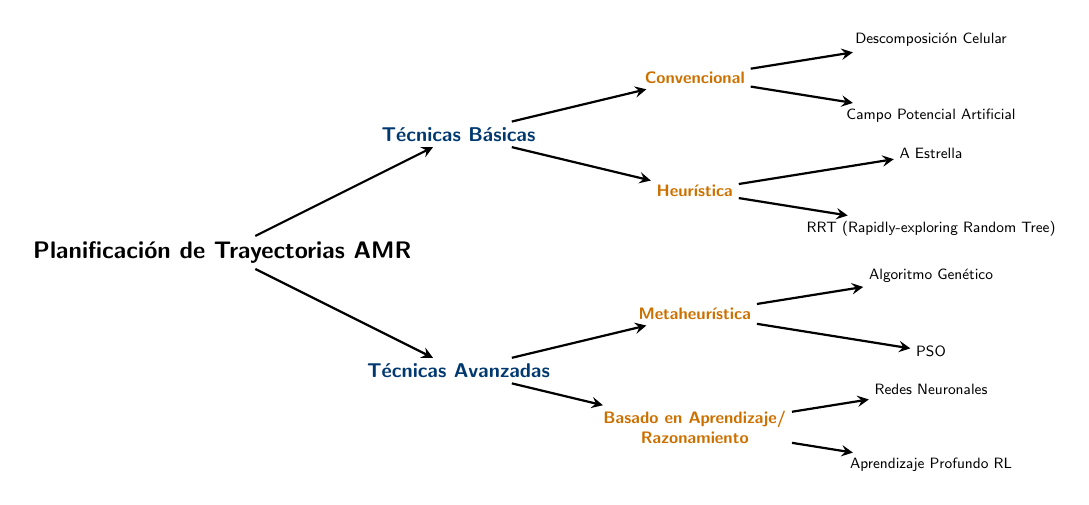
\begin{tikzpicture}[scale=0.6, transform shape,
      node distance=5cm and 3cm,
      every node/.style={align=center},
      font=\sffamily
  ]
  % Level 1 (root)
  \node[level1] (root) {Planificación de Trayectorias AMR};

  \node[level2] (basic) at ([xshift=5cm, yshift=2.5cm]root) {Técnicas Básicas};
  \node[level2] (advanced) at ([xshift=5cm, yshift=-2.5cm]root) {Técnicas Avanzadas};

  \node[level3] (conventional) at ([xshift=5cm, yshift=1.2cm]basic) {Convencional};
  \node[level3] (heuristic) at ([xshift=5cm, yshift=-1.2cm]basic) {Heurística};

  \node[level3] (metaheuristic) at ([xshift=5cm, yshift=1.2cm]advanced) {Metaheurística};
  \node[level3] (learning) at ([xshift=5cm, yshift=-1.2cm]advanced) {Basado en Aprendizaje/\\Razonamiento};

  \node[endpoint] (s1) at ([xshift=5cm, yshift=0.8cm]conventional) {Descomposición Celular};
  \node[endpoint] (s2) at ([xshift=5cm, yshift=-0.8cm]conventional) {Campo Potencial Artificial};

  \node[endpoint] (s3) at ([xshift=5cm, yshift=0.8cm]heuristic) {A Estrella};
  \node[endpoint] (s4) at ([xshift=5cm, yshift=-0.8cm]heuristic) {RRT (Rapidly-exploring Random Tree)};

  \node[endpoint] (s5) at ([xshift=5cm, yshift=0.8cm]metaheuristic) {Algoritmo Genético};
  \node[endpoint] (s6) at ([xshift=5cm, yshift=-0.8cm]metaheuristic) {PSO};

  \node[endpoint] (s7) at ([xshift=5cm, yshift=0.8cm]learning) {Redes Neuronales};
  \node[endpoint] (s8) at ([xshift=5cm, yshift=-0.8cm]learning) {Aprendizaje Profundo RL};

  % Connect nodes with arrows
  \draw[arrow] (root) -- (basic);
  \draw[arrow] (root) -- (advanced);

  \draw[arrow] (basic) -- (conventional);
  \draw[arrow] (basic) -- (heuristic);

  \draw[arrow] (advanced) -- (metaheuristic);
  \draw[arrow] (advanced) -- (learning);

  \draw[arrow] (conventional) -- (s1);
  \draw[arrow] (conventional) -- (s2);

  \draw[arrow] (heuristic) -- (s3);
  \draw[arrow] (heuristic) -- (s4);

  \draw[arrow] (metaheuristic) -- (s5);
  \draw[arrow] (metaheuristic) -- (s6);

  \draw[arrow] (learning) -- (s7);
  \draw[arrow] (learning) -- (s8);

  \end{tikzpicture}
\end{frame}

\begin{frame}{Algoritmo RRT}
  \begin{figure}
    \begin{center}
      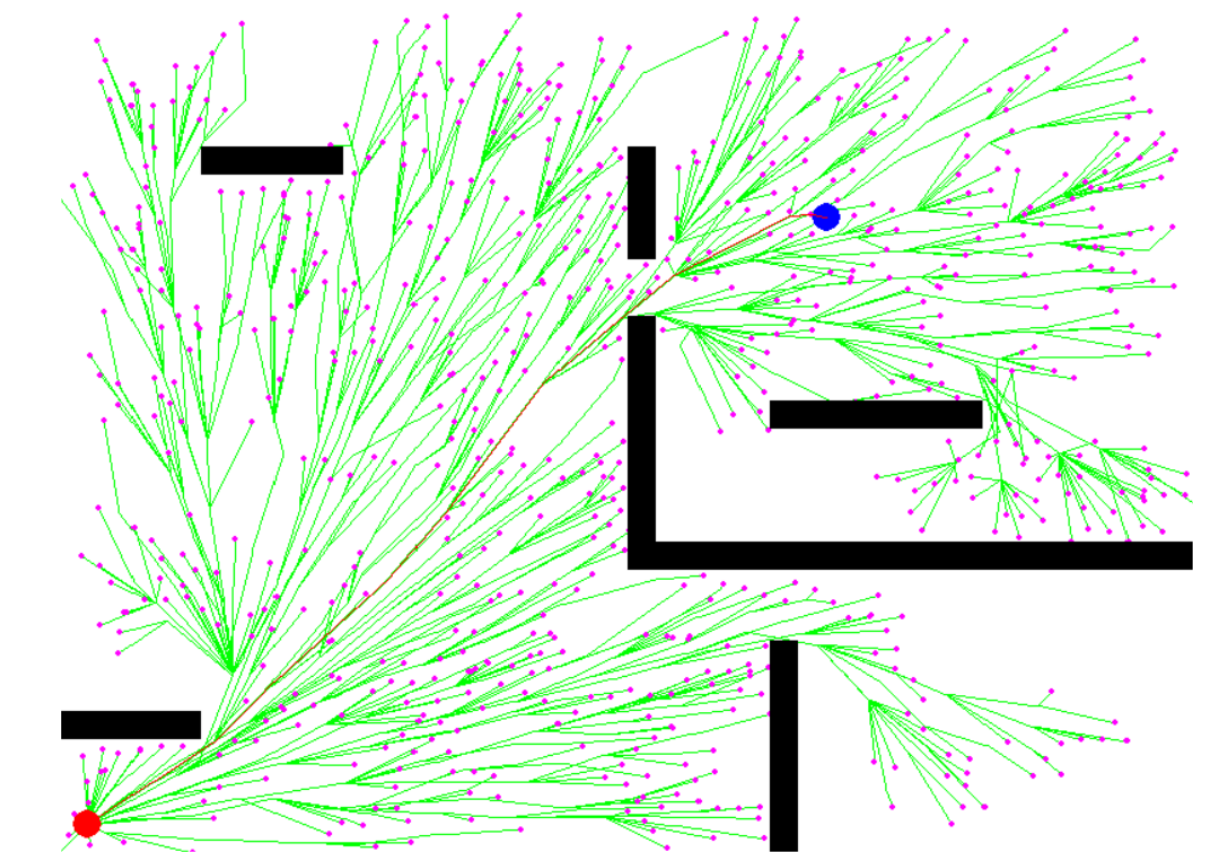
\includegraphics[width=0.95\textwidth]{figures/rrt.png}
    \end{center}
    \caption{Algoritmo RRT (Rapidly-exploring Random Tree)}\label{fig:rrt}
  \end{figure}
\end{frame}

\begin{frame}{Virtual Teleoperation System for Mobile Manipulator Robots Focused on Object Transport and Manipulation \scriptsize{Fernando J. Pantusin, Christian P. Carvajal, Jessica S. Ortiz and Víctor H. Andaluz}}

  Se presenta un sistema de teleoperación virtual para robots manipuladores móviles enfocado en el transporte y manipulación de objetos.\\[5pt]

  \textbf{Problemáticas:}
  \begin{itemize}
    \item Adquisición de conocimiento en el modelaje y control de robots móviles.
  \end{itemize}

  \textbf{Propuestas:}
  \begin{itemize}
    \item Sistema de teleoperación para la enseñanza y aprendizaje.
    \item Modelo cinemático y dinámico para robot móvil omnidireccional con manipulador.
  \end{itemize}

  \textbf{Resultado:}
  \begin{itemize}
    \item Entorno virtual con realismo físico significativo.
  \end{itemize}
\end{frame}

\begin{frame}{Sistema Virtual}
  \begin{figure}
    \begin{center}
      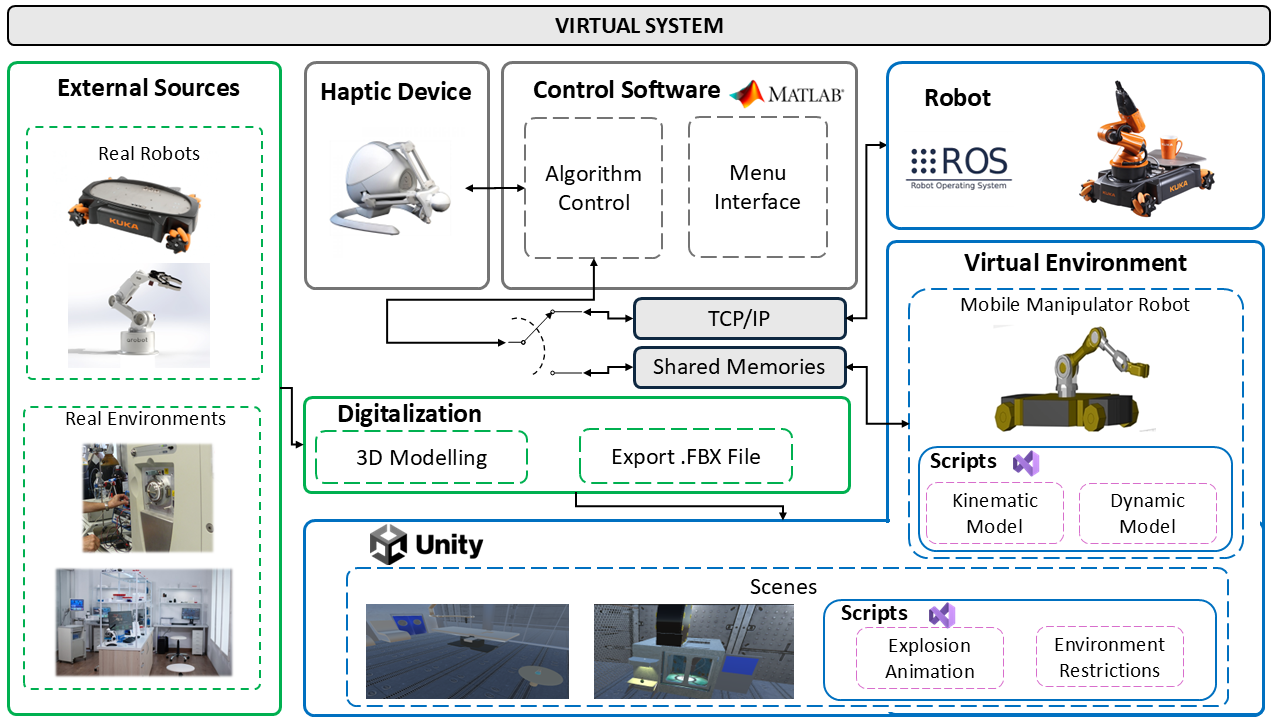
\includegraphics[width=0.7\textwidth]{figures/virtual-system.png}
    \end{center}
    \caption{Sistema Virtual de Teleoperación}\label{fig:virtualsystem}
  \end{figure}
\end{frame}

\begin{frame}{A General Inverse Kinematic Formulation and Control Schemes for  Omnidirectional Robots \scriptsize{Indrazno Siradjuddin, Gillang Al Azhar, Sapto Wibowo, Ferdian Ronilaya, Cahya Rahmad and ROHADI Erfan}}
  Se presenta una formulación cinemática inversa genérica para robots móviles omnidireccionales con ruedas omni y mecanum.\\[5pt]

  \textbf{Problemáticas:}
  \begin{itemize}
    \item Formulación cinemática genérica para modelar robots móviles omnidireccionales que utilizan tipos de ruedas omni y mecanum.
  \end{itemize}

  \textbf{Propuestas:}
  \begin{itemize}
    \item La formulación puede utilizarse para cualquier numero \(n\) de ruedas del robot.
  \end{itemize}

  \textbf{Resultado:}
  \begin{itemize}
    \item Se obtuvo la formulación de la cinemática inversa generalizada.
  \end{itemize}
\end{frame}

\begin{frame}{Especificaciones}
  Parámetros cinemáticos de tres ruedas omni y cuatro ruedas mecanum.
  
  \begin{table}[htbp]
      \centering
      \renewcommand{\arraystretch}{1.2}
      \begin{tabular}{|c|c|c|c|c|}
      \hline
      \multirow{2}{*}{Número de Ruedas} & \multicolumn{2}{c|}{Tres ruedas omni} & \multicolumn{2}{c|}{Cuatro ruedas mecanum} \\
      \cline{2-5}
       & $\alpha_i$ & $\beta_i$ & $\alpha_i$ & $\beta_i$ \\
      \hline
      $W_1$ & $150^{\circ}$ & $0^{\circ}$ & $0^{\circ}$ & $-45^{\circ}$ \\
      \hline
      $W_2$ & $-90^{\circ}$ & $0^{\circ}$ & $0^{\circ}$ & $45^{\circ}$ \\
      \hline
      $W_3$ & $30^{\circ}$ & $0^{\circ}$ & $0^{\circ}$ & $-45^{\circ}$ \\
      \hline
      $W_4$ & - & - & $0^{\circ}$ & $45^{\circ}$ \\
      \hline
      \end{tabular}
      \caption{Configuración de ángulos para ruedas omni y mecanum.}
      \label{tabla:ruedas}
  \end{table}
\end{frame}

\end{document}
